% This is "sig-alternate.tex" V1.9 April 2009
% This file should be compiled with V2.4 of "sig-alternate.cls" April 2009
%
% This example file demonstrates the use of the 'sig-alternate.cls'
% V2.4 LaTeX2e document class file. It is for those submitting
% articles to ACM Conference Proceedings WHO DO NOT WISH TO
% STRICTLY ADHERE TO THE SIGS (PUBS-BOARD-ENDORSED) STYLE.
% The 'sig-alternate.cls' file will produce a similar-looking,
% albeit, 'tighter' paper resulting in, invariably, fewer pages.
%
% ----------------------------------------------------------------------------------------------------------------
% This .tex file (and associated .cls V2.4) produces:
%       1) The Permission Statement
%       2) The Conference (location) Info information
%       3) The Copyright Line with ACM data
%       4) NO page numbers
%
% as against the acm_proc_article-sp.cls file which
% DOES NOT produce 1) thru' 3) above.
%
% Using 'sig-alternate.cls' you have control, however, from within
% the source .tex file, over both the CopyrightYear
% (defaulted to 200X) and the ACM Copyright Data
% (defaulted to X-XXXXX-XX-X/XX/XX).
% e.g.
% \CopyrightYear{2007} will cause 2007 to appear in the copyright line.
% \crdata{0-12345-67-8/90/12} will cause 0-12345-67-8/90/12 to appear in the copyright line.
%
% ---------------------------------------------------------------------------------------------------------------
% This .tex source is an example which *does* use
% the .bib file (from which the .bbl file % is produced).
% REMEMBER HOWEVER: After having produced the .bbl file,
% and prior to final submission, you *NEED* to 'insert'
% your .bbl file into your source .tex file so as to provide
% ONE 'self-contained' source file.
%
% ================= IF YOU HAVE QUESTIONS =======================
% Questions regarding the SIGS styles, SIGS policies and
% procedures, Conferences etc. should be sent to
% Adrienne Griscti (griscti@acm.org)
%
% Technical questions _only_ to
% Gerald Murray (murray@hq.acm.org)
% ===============================================================
%
% For tracking purposes - this is V1.9 - April 2009
\documentclass{sig-alternate}

\usepackage{tabularx}
\usepackage{xspace,siunitx}
\usepackage{hyperref}

\usepackage{tikz, pgfplots}
\pgfplotsset{compat=newest}

\usepackage{subfigure,booktabs}

\usetikzlibrary{fit}
\usetikzlibrary{backgrounds}
\usetikzlibrary{trees}

\newcommand{\darkvr}{\textsc{DarkVR}\xspace}

\begin{document}
%
% --- Author Metadata here ---
%\conferenceinfo{ }
%\CopyrightYear{ } % Allows default copyright year (20XX) to be over-ridden -
% IF NEED BE.
%\crdata{ }  % Allows default copyright data
% (0-89791-88-6/97/05) to be over-ridden - IF NEED BE.
% --- End of Author Metadata ---

\title{DarkVR: The Virtual Blind Reality}
%\subtitle{[Extended Abstract]
%
% You need the command \numberofauthors to handle the 'placement
% and alignment' of the authors beneath the title.
%
% For aesthetic reasons, we recommend 'three authors at a time'
% i.e. three 'name/affiliation blocks' be placed beneath the title.
%
% NOTE: You are NOT restricted in how many 'rows' of
% "name/affiliations" may appear. We just ask that you restrict
% the number of 'columns' to three.
%
% Because of the available 'opening page real-estate'
% we ask you to refrain from putting more than six authors
% (two rows with three columns) beneath the article title.
% More than six makes the first-page appear very cluttered indeed.
%
% Use the \alignauthor commands to handle the names
% and affiliations for an 'aesthetic maximum' of six authors.
% Add names, affiliations, addresses for
% the seventh etc. author(s) as the argument for the
% \additionalauthors command.
% These 'additional authors' will be output/set for you
% without further effort on your part as the last section in
% the body of your article BEFORE References or any Appendices.

\numberofauthors{1} %  in this sample file, there are a *total*
% of EIGHT authors. SIX appear on the 'first-page' (for formatting
% reasons) and the remaining two appear in the \additionalauthors section.
%
\author{
% You can go ahead and credit any number of authors here,
% e.g. one 'row of three' or two rows (consisting of one row of three
% and a second row of one, two or three).
%
% The command \alignauthor (no curly braces needed) should
% precede each author name, affiliation/snail-mail address and
% e-mail address. Additionally, tag each line of
% affiliation/address with \affaddr, and tag the
% e-mail address with \email.
%
% 1st. author
\alignauthor
Tom Brosch\\
       \affaddr{MS/MRI Research Group}\\
      	\affaddr{University of British Columbia}\\
		\affaddr{Suite \#203 2386 East Mall}\\
		\affaddr{Vancouver, BC, V6T 1Z3}\\ 
       \email{tombr@msmri.medicine.ubc.ca}
}
% There's nothing stopping you putting the seventh, eighth, etc.
% author on the opening page (as the 'third row') but we ask,
% for aesthetic reasons that you place these 'additional authors'
% in the \additional authors block, viz.
\date{\today}
% Just remember to make sure that the TOTAL number of authors
% is the number that will appear on the first page PLUS the
% number that will appear in the \additionalauthors section.

\maketitle

\begin{abstract}

This paper introduces \darkvr, a virtual environment designed to give the blind
experience to sighted people. In \darkvr, people can explore two different
environments, relying complete on hearing. Thereby, \darkvr provides not only a
fun challenge, it also helps to raise awareness for the problems of visually
impaired in an engaging manner. To give the best 3D audio experience,
state-of-the-art sound engines are combined with head tracking to let the
sounds appear static in a 3D space. A preliminary user-study with 6 subjects
showed the potential and future challenges to make \darkvr a success.

\end{abstract}

% A category with the (minimum) three required fields
\category{H.5.2}{Information Interfaces and Presentation}{User
Interfaces}[auditory feedback]
%A category including the fourth, optional field follows...

%\terms{Theory}

\keywords{Virtual reality, 3D audio, blind, dialogue in the dark}

\section{Introduction}

The project aims to create a virtual reality environment without visual cues and
without substituting visual cues by auditory cues (e.g. playing the sound of a
creaking door when you stand right in front of a door). The aim of the project
is to create and experience a virtual world as close as possible to
how non-sighted people would experience the real world. Therefore, two virtual
worlds were created that can be explored relying on hearing only.

The state-of-the-art 3D audio engine FMOD\cite{fmod} was combined with magnetic
head-tracking in order to let the sounds appear static in 3D, independent of
head movement. To further assist navigation, the user can use a virtual cane
which provides auditory feedback when hitting objects in the virtual
environment. Figure~\ref{fig:intro} shows the system in use.

\begin{figure}
\centering
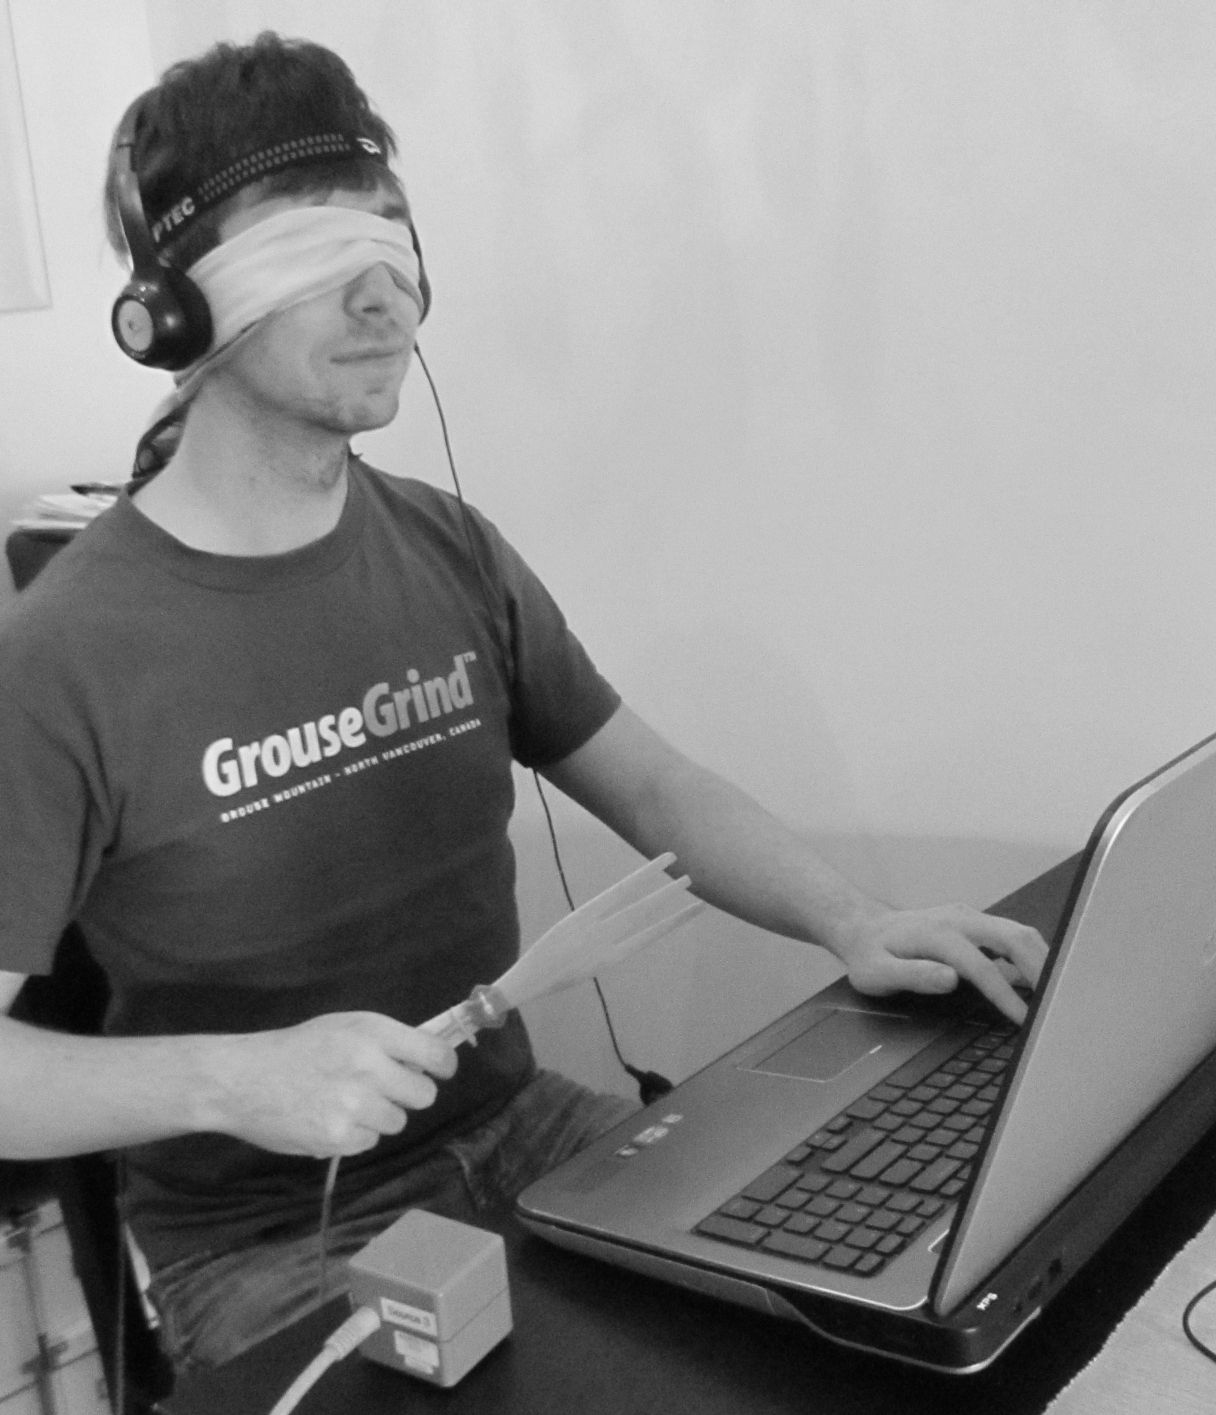
\includegraphics[width=0.75\columnwidth]{images/intro3}
\caption{The \darkvr system. User experiencing the zoo environment blindfolded
completely relying on hearing.}
\label{fig:intro}
\end{figure}

The remainder of the paper is structured as follows: Section~\ref{sec:related}
briefly reviews related work. The whole system is then introduced in
section~\ref{sec:method}. The design of the user study is described in
section~\ref{sec:study}, followed by the evaluation of the results.
Section~\ref{sec:conclusion} concludes the paper with a discussion of the
results and future work.

\section{Related Work}
\label{sec:related}
This work is most closely related to the \textsc{Dialogue in the Dark}
project\cite{dialog}. \textsc{Dialogue in the Dark} is an exhibition which lets
sighted people experience the world of visually impaired and, thereby, raises
awareness for the problems non-sighted are faced everyday while navigate
through the world. Since the created environments are replicas build in an
indoor space, the scenarios that can be rebuild are very limited. A
virtual reality can help bringing the blindness-experience to scenarios that are
too expensive to rebuild (e.g. navigating through an entire city) or too
dangerous (e.g. due to traffic).

The work is also related to video games for blinds. Video games for blinds can
be roughly classified into two categories: (1) games, which were initially
designed for blinds, and (2) games which have been made accessible to blinds.
Games of the first category often either use a combination of a
narrator, which introduces and describes a new scene, and auditory feedback,
which helps the user to navigate through the virtual environment (e.g. ``Der Tag
wird zur Nacht''\cite{dertag}); or use sound as the primary gaming concept (e.g.
``AudiOdyssey''\cite{audiodyssey}).

There has also been a great amount of research in how to make games accessible
for disabled people (e.g. \cite{chile, terraformers, secondlife,
tankcommander}). See \cite{survey} for a survey of accessible games. A common
method is to replace visuals with audio. This can be done on different levels of
abstraction. Audio cues are the least abstract way of replacing visuals with
audio. Audio cues are sounds that an object would make in the real world (e.g.
footsteps of a walking person). Auditory Icons or ear cons are sounds which are
associated with an object, even though the object would not make this sound in
the current situation (e.g. playing the sound of a creaking door when you stand
in front of it, even if the door is not moving). Sonification is used to
translate physical properties of an object into sound. These sounds are usually
artificial. Properties like pitch or frequency are used to represent other
properties like distance.

In contrast to the many attempts to making a virtual world accessible for the
blinds, this project aims to create an experience which is as closed as
possible to the real experience of blindness. Therefore, accessibility methods
like auditory icons/ear cons and sonifications are not used on purpose. Instead,
the user navigates through the world relying on 3D binaural audio and devices
like a virtual long cane or a virtual GPS localizer. \darkvr, therefore,
does not only give the possibility to experience blindness, it also gives the
possibility to try out imaginary devices that might help blinds in the
future to navigate and orientate in the real world.

\section{Implementation}
\label{sec:method}
\darkvr is a virtual environment that simulates the perception of the
world of visually impaired. An overview of the setup is shown in
figure~\ref{fig:setup}. The system consists of a laptop, a magnetic field
source, two trackers (one for the head and one for the virtual cane),
headphones, and a sleep mask or a scarf. The world is also visualized in 3D in
order to enable other people to provide assistance to the user.

\begin{figure}
\centering
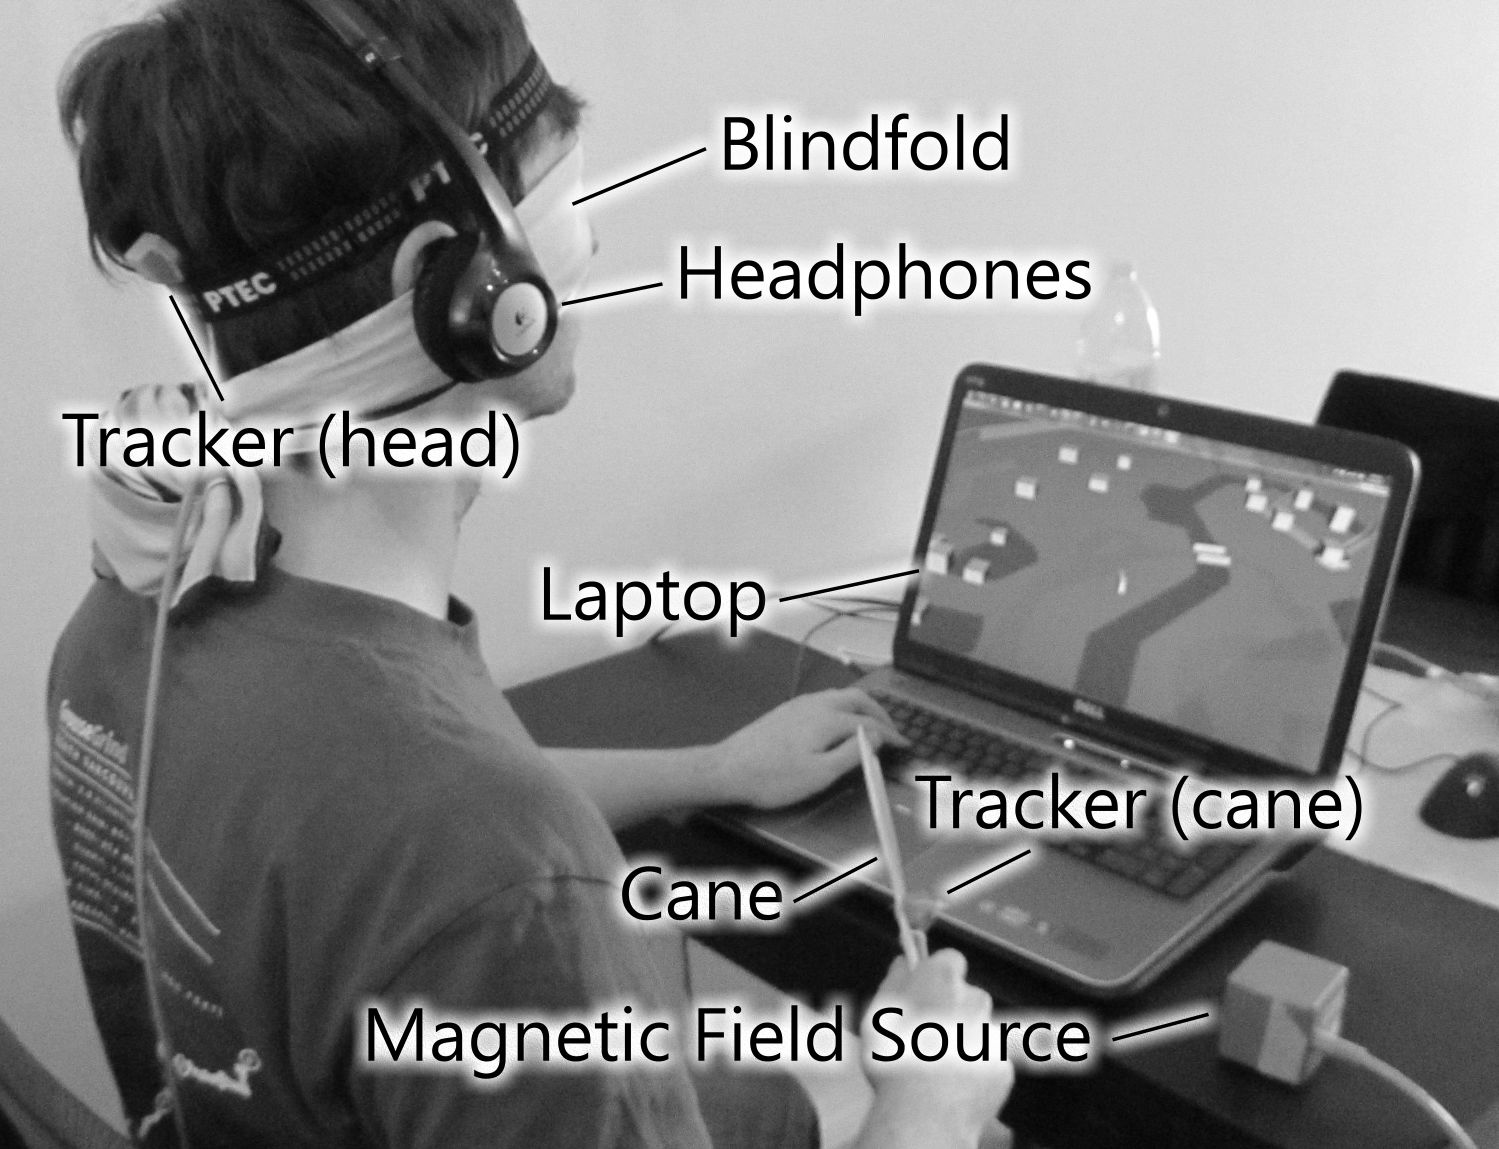
\includegraphics[width=\columnwidth]{images/details_sw}
\caption{The \darkvr setup consists of a blindfold, headphones for 3D audio
using head-related transfer functions (HRTFs), magnetic tracker for the head,
cane with attached magnetic tracker, magnetic field source, and a laptop}
\label{fig:setup}
\end{figure}

This section describes the implementation of \darkvr. First, the design of the
software is briefly introduces, followed by the design of the soundscape. This
section concludes with a description of how virtual worlds can be modelled
followed by a brief description of two examples environments: a zoo and an
apartment.

\subsection{Software Design}

\subsubsection{Overview}

The software builds upon OpenSceneGraph\cite{osg}, a high level 3D
graphics library based on OpenGl\cite{opengl}. All 3D models of the world, the avatar,
the cane, and various 3D sound sources are organized in a scene graph. The basic
structure of the scene graph is shown in figure~\ref{fig:graph}. It is worth
noting that the body is further divided into the main body part (Body Node) and
the head part (Head Node). This division allows for head motion relative to the
body. Once the scene graph is loaded from a 3D model file, the program runs in a
continues game loop. During each cycle, user input through the keyboard and the
trackers is processed and compiled into scene graph and soundscape modification.

%Game loop. Some components make changes to the scene graph. Afterwards, the
%scenegraph is traversed in order to create the outputs. Show how the scene
% graph looks like. Use open scene graph for 3D rendering. Content is provided
% using
%collada 3D models. Sound and material properties are encoded.

\begin{figure}
\centering
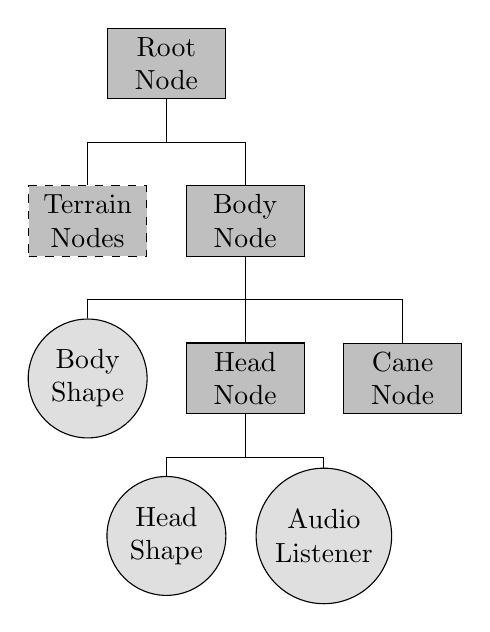
\begin{tikzpicture}[level distance=2cm, sibling distance=2cm]
%[grow via three points={
%one child at (0,-2) and two children at (-1,-3) and (1,-3)}, level distance=-1]

\tikzstyle{osgnode}=[align=center,draw=black, minimum
width=1.5cm,fill=lightgray]
\tikzstyle{osgelement}=[align=center,shape=circle,draw=black,fill=lightgray!50]

\node[osgnode] {Root\\Node}
[edge from parent fork down]
child {node[osgnode,dashed] {Terrain\\Nodes}}
child {node[osgnode] {Body\\Node}
	child {node[osgelement] {Body\\Shape}}
	child {node[osgnode] {Head\\Node}
		child {node[osgelement] {Head\\Shape}}
		child {node[osgelement] {Audio\\Listener}}
	}
	child {node[osgnode] {Cane\\Node}}
};
\end{tikzpicture}

\caption{Basic structure of the scene graph. There is a dedicated node for the
head. This allows for head motion independent of the whole body motion. The
audio listener is attached to the head.}
\label{fig:graph}
\end{figure}

\subsubsection{Tracker calibration}

In order to ease the use of the system, the head tracker can be attached to any
location on the head. The head tracker is than automatically calibrated when
the system starts. Therefore, the head has to be in a normal position looking
straight when the system starts. The initial tracker position and orientation at
the start of the system is later used to calculate the head movement relative to
the initial position.

Since the position of the cane tracker relative to the cane is fixed, this
tracker does not need to be calibrated every time the system starts. In order to
be independent of the placement of the magnetic field source, the position of
the cane relative to the body is normalized using the initial head position.

\subsubsection{Controls}

The avatar can be moved using the keyboard. The basic hotkeys are summarized in
table~\ref{tab:keys}. The user can choose between two different rotation modes:
discrete and continuous. In discrete mode, the user rotates around a certain
amount (e.g \ang{45}) when hitting a rotation key. The user has to release and
press again the key in order to further rotate. In order to avoid collision
while rotating, the avatar is shaped like a cylinder. This makes navigation
easier, once the user has hit a wall.

\begin{table}[tb]
\centering
\caption{Keyboard controls of the avatar. The amount of rotation can be
controlled from the command line. It is also possible to switch between
continuous and discrete rotations.}
\label{tab:keys}
\vspace{1em}
\begin{tabular}{@{}cl@{}}
\bottomrule
Key & Action\\
\cmidrule(r){1-1} \cmidrule(l){2-2}
\texttt{W} & Moves the avatar forwards\\
\texttt{A} & Moves the avatar to the left\\
\texttt{S} & Moves the avatar backwards\\
\texttt{D} & Moves the avatar to the right\\
\texttt{Q} & Rotates the avatar to the left\\
\texttt{E} & Rotates the avatar to the right\\
\texttt{ESC} & Quit the program\\
\bottomrule
\end{tabular}
\end{table}

The virtual cane can be controlled with the wooden wand. The virtual cane
obeys the full range of 6 degrees of freedom.

\subsection{Sound Design}

The first part of \darkvr's sound engine is a wrapper around the FMOD Sound
System\cite{fmod}, which is used to output 3D spatial audio. FMOD provides
realistic 3D audio using head-related transfer functions (HRTFs). It also
calculates realistic audio occlusion using the 3D geometric model of the world.
Therefore, 3D models described by the scene graph are translated to
FMOD's internal geometry representation.

The second part of the sound engine is a powerful sound event manager, which
queues and triggers randomized sound events. The time between to events is drawn
form a uniform distribution. The the minimum and maximum delay between two
occurrences can be specified individually for every sound event.

The sound engine also handles triggered sound events that are the result of the
interaction of the avatar or the cane with the world. When the avatar moves, a
footstep sound is played which depends on the material of the ground under the
avatar. A collisions of the cane with the world trigger a sound as well, which
depends on the material of the hit object.

\subsection{World Design}

The 3D world can be modelled using any 3D modelling program that can output 3D
models in a format that can be read with OpenSceneGraph. The models of the first
prototype were created using SketchUp 3D and exported as Collada 3D models.
Since most modelling programs are not made for sound design, sounds are modelled
as 3D objects, too. Sound source properties (e.g. the audio file name, the
minimum distance, or the volume) and audio material properties (like wooden,
grass, water, \dots) are encoded in the name of the object. The two created
worlds from a bird's-eye view are shown in figure~\ref{fig:levels}.

\subsubsection{The Zoo}

The terrain of the zoo is a remodelling of parts of the Zoo
Leipzig\cite{zooleipzig}. The placement of animals are arbitrary. The zoo
features different birds, elephants, tigers, monkeys, hippopotamus, sea lions,
and frogs, with 3 to 7 different sounds per animal. The ground is made of 5
different materials (parkway, grass, hollow wood, stone, and water). Each
material comes with a distinctive footstep and cane hit sound.

\subsubsection{The Apartment}

The apartment consists of 8 different rooms and a basic outeriour. Different
ground or floor types are carpet, concrete, linoleum, tiles, and grass.
Some rooms have a sound attached to it. There is one room with a playing radio that can be heard
throughout the apartment. Rooms can not be identified by the ground material
alone since some rooms share the same flooring. E.g. the bathroom and the
kitchen are both tiled but the fridge is only audible in the kitchen.

%\usepackage{graphics} is needed for \includegraphics
\begin{figure*}[tb]
  \centering
  \subfigure[One part of the Zoo Leipzig]{
  	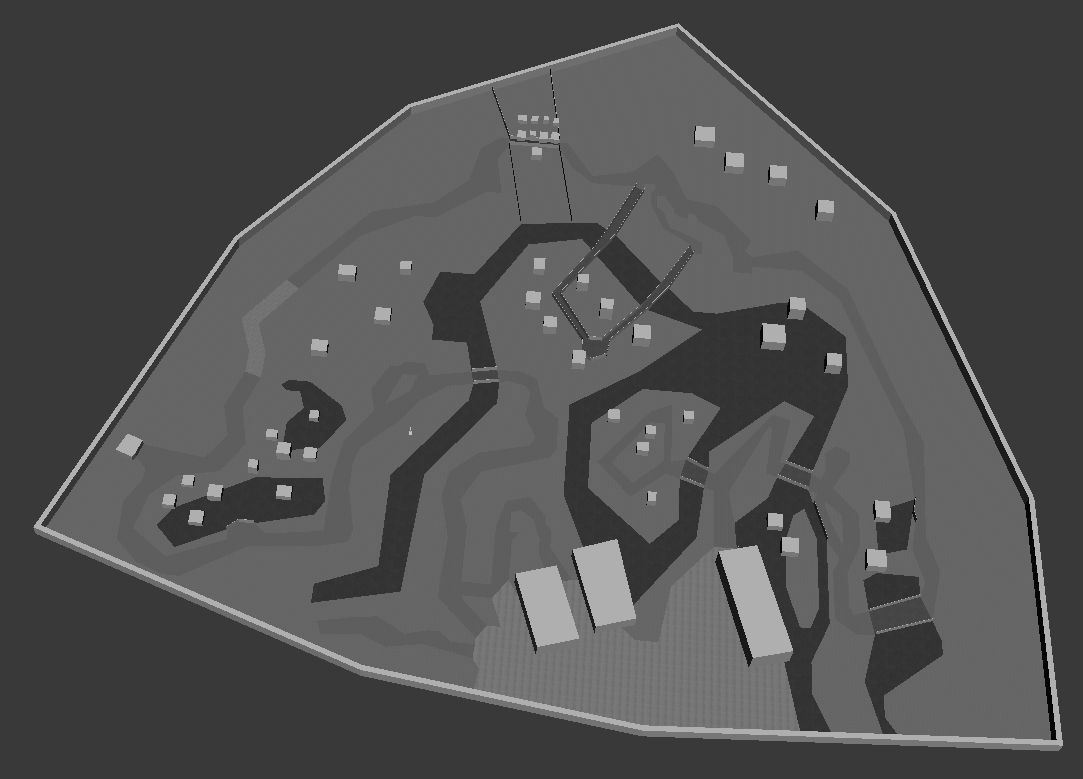
\includegraphics[height=0.7\columnwidth]{images/zoo_sw}
  }
  %\quad
  \subfigure[The apartment]{
  	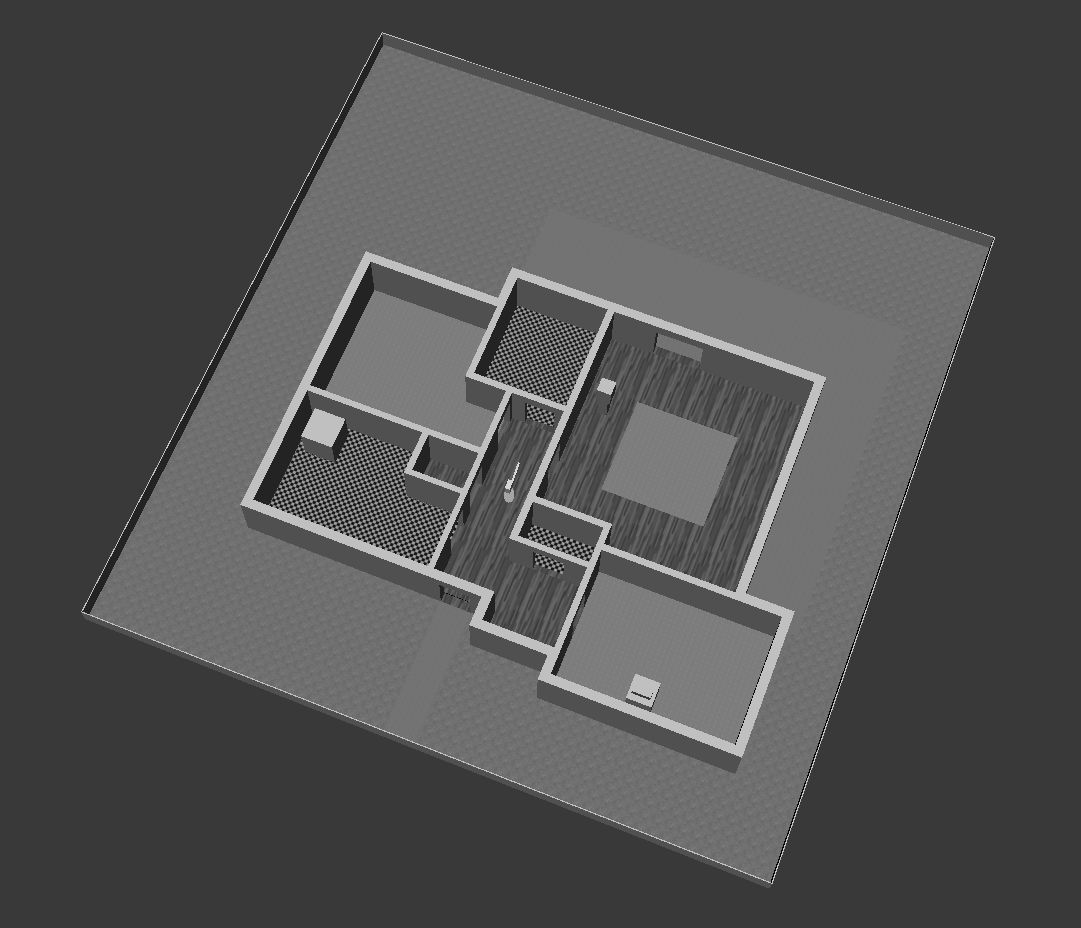
\includegraphics[height=0.7\columnwidth]{images/apartment_sw}
  }
  \caption{The two created environments from the bird's-eye view. Small blocks
  in the zoo represent the different animals.}
  \label{fig:levels}
\end{figure*}

\section{Study Design}
\label{sec:study}
The objective of study was to evaluate if the use of the program can raise
awareness for the problems of visually impaired. Therefore, a questionnaire was
used to asses the awareness before and after the subjects had solved a few
tasks within \darkvr. 

\subsection{Participants}

The test group of the user study consisted of 6 participants (5 male, 1 female)
in the age between 20 and 40 years. All of them were familiar with computer
games in general. None of them had experience with visually impaired people.

\subsection{Study Procedure}

After a short introduction, each participant had the chance to get familiar with
the control of the program. Therefore, they were asked to move freely in the zoo
without the blindfold and to get familiar with different footstep and cane hit
sounds. Then, the participants were asked to put on the blindfold.

The first task was to follow a trail in the zoo. This task required to listen to
footstep sounds in order to detect when the avatar leaves the trail and to use
the cane in order to distinguish a bend to the right from a bend to the left.
The second task was to find the elephants in the zoo and to identify one more
animal. The subjects were allowed to move freely in the zoo without having to
stay on the trail. ``Looking around'' was helpful in order to localize sounds
better in 3D.

The last task took place in the apartment. In contrast to the zoo scene, the
rotation mode was changed to discrete, which simplifies the navigation in mainly
orthogonal environments. In the first step, the participants were guided through
the apartment with simple voice commandos from the tester. They were also told
in which room they are in. After the introduction, the participants were guided
into different rooms and they were asked to tell, in which room they are in. The
performance of the subjects in all three tasks was not measured. They were
merely used to let the subjects experience the virtual environment in a more
challenging setting.

\subsection{The Questionnaire}

The questionnaire was divided into three parts: personal information, questions
that were to be completed before and questions that were to be completed after
the experiment. In both parts, subjects were asked to rate the difficulty of the
following tasks for visually impaired on a 5 level scale: ``crossing a
street'', ``walking in a park'', ``navigating in an unknown apartment'', and ``navigating in a known
apartment''. They were also asked to imagine, which other tasks might be
difficult for visually impaired. A second set of questions was used to identify
the importance of several cues for the navigation.

\section{Results}
\label{sec:results}

The usability of the program was rated as easy and intuitive by all subjects.
Difficulties to solve other tasks are hence mainly caused by the lack of visual
feedback. The quality of the implementation (e.g. localization of 3D
sounds) was rated as good by most participants.

In order to measure if the use of the program can raise the awareness of the
problems of visually impaired, the rated difficulty for certain tasks before and
after the experiment were compared. The result of the comparison is shown in
figure~\ref{fig:results}. Most tasks were rated more difficult after the
experiment by most subjects. However, the variation between subjects is too high
to conclude that the increase in rated difficulty is statistically significant.
The ``navigation in an unknown apartment'' task was even rated easier after the
experiment. A possible explanation for this result is, that the task might have
been too simple. In previous tests, the navigation in the apartment without help
was perceived as being to difficult. Therefore, the participants were guided
throughout the entire task using voice commands, which might have decreased the
difficulty too much.

\begin{figure}[tb]
\centering

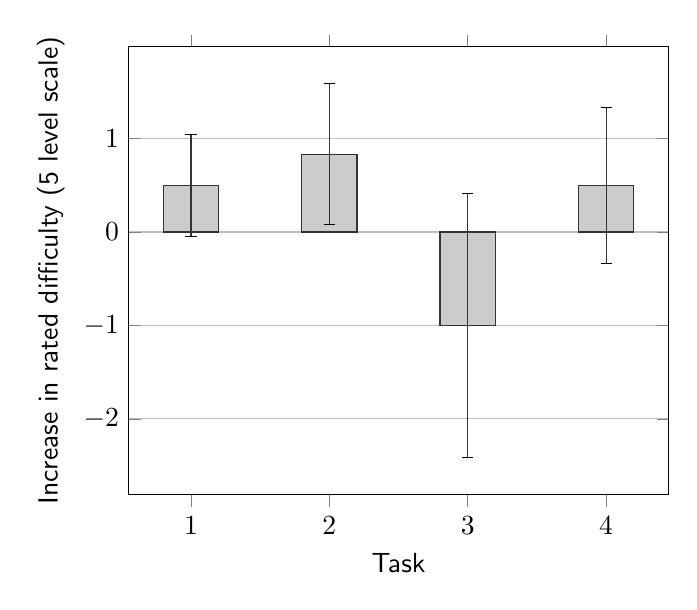
\begin{tikzpicture}

\tikzstyle{every node}+=[font=\sffamily]

\begin{axis}[
ymajorgrids=true, yminorgrids=true,
ybar,
xtick=data,
bar width=20pt,
enlarge x limits=0.15,
xlabel={Task},
ylabel={Increase in rated difficulty (5 level scale)}
]

\addplot[fill=black!20,draw=black!80,
error bars/.cd, y explicit, y dir=both] coordinates {
(1,0.5)+-(0,0.547722558)
(2,0.833333333)+-(0,0.752772653)
(3,-1)+-(0,1.414213562)
(4,0.5)+-(0,0.836660027)
};

\end{axis}

\end{tikzpicture}

\caption{Change of rated difficulty on a 5 level scale of the following tasks:
(1) ``crossing a street'', (2) ``walking in a park'', (3) ``navigating in an unknown apartment'',
and (4) ``navigating in a known apartment''. The standard deviation is indicated
by the error bars. The standard deviation is too large to detect a significant
increase in the rated difficulty.}

\label{fig:results}
\end{figure}

4 of 6 subjects have identified more difficult tasks for visually impaired after
the experiment. While some of them are directly related to the newly gained
experience (e.g. subject 4 answered after the experiment, that it is difficult
for visually impaired to operate technical equipment like computers), others
could also be explained by the fact, that the participants merely had more time to
think about potential problems.

The last questions were posed to help improving future version of the program.
Therefore, the subjects were asked which cues they think are important for
navigation. Most subjects agreed that force-feedback of the cane and vibration
of the cane on different ground would be very helpful.

\section{Discussion and Future Work}
\label{sec:conclusion}

The evaluation of the user study has revealed that even though it is still
unclear, if \darkvr can help to increase awareness for the problems of visually
impaired, the approach bears some potential. However, auditory cues alone are
not sufficient to facilitate a satisfying navigation in an unknown environment
without visual cues. I anticipate that the use of 6 degree force-feedback
devices like the PHANTOM\cite{phantom}, will greatly increase the possibility to
navigate freely without too much assistance, in order to provide a more
realistic blind experience. The enables the implementation of more realistic
scenarios which are better suited to raise awareness of the problems of visually
impaired.

\section{Acknowledgments}
I would like to thank Dr. Sidney Fels for guidance throughout the entire project
and the MAGIC lab for providing the magnetic trackers.

%  The following two commands are all you need in the initial runs of your .tex
% file to produce the bibliography for the citations in your paper.
\bibliographystyle{abbrv}
\bibliography{sigproc}  % sigproc.bib is the name of the Bibliography in this
\end{document}
